\pdfminorversion=7%
\documentclass[aspectratio=169,mathserif,notheorems]{beamer}%
%
\xdef\bookbaseDir{../../bookbase}%
\xdef\sharedDir{../../shared}%
\RequirePackage{\bookbaseDir/styles/slides}%
\RequirePackage{\sharedDir/styles/styles}%
%
\gdef\searchSpace{\ensuremath{\mathbb{X}}}%
\gdef\sespel{\ensuremath{x}}%
\gdef\opti#1{\ensuremath{#1^{\star}}}%
%
%% Print an algorithm box around something.
\protected\gdef\algobox#1#2{\resizebox{#1\paperwidth}{!}{%
\bgroup%
\fboxsep=0pt%
\fboxrule=2pt%
\mbox{\fcolorbox{white}{white}{\bgroup%
\fboxsep=2pt%
\fboxrule=2pt%
\mbox{\fcolorbox{hfuu-red!80}{hfuu-orange!60}{%
\mbox{#2}%
}}\egroup%
}}%
\egroup}}%
%
%
\title{\mbox{Frequency Fitness Assignment} as a \mbox{Research Direction}}%
%
\begin{document}%
\startPresentation%
%
\section{Introduction}%
%
\begin{frame}%
\frametitle{Introduction}%
\begin{itemize}%
%
\item Our team has two general research directions:~Optimization\cite{W2009GOATAA} and \glsFull{AI}.%
%
\item<2-> My students and I are members of the \alert{Optimization Direction}.%
%
\item<3-> Today, I therefore want to first give a short introduction into the field of optimization, before delving into one of our concrete research topics, namely \glsFull{algoFFA}.%
%
\end{itemize}%
\end{frame}%
%
\section{Research Field: Optimization}%
%%
\begin{frame}[t]%
\frametitle{What is Optimization?}%
\begin{itemize}%
\only<-1>{\item There are two ways to look at optimization.}%
\only<-2>{\item<2-> The economic view.}%
\item<3-> The mathematical view.%
\end{itemize}%
\locateGraphic{2}{width=0.75\paperwidth}{\sharedDir/graphics/optimization_views/optimization_views_1}{0.125}{0.3}%
\locateGraphic{3}{width=0.75\paperwidth}{\sharedDir/graphics/optimization_views/optimization_views_2}{0.125}{0.3}%
\end{frame}%
%
\begin{frame}%
\frametitle{Example: Function Optimization}%
\locate{}{%
\parbox{0.373\paperwidth}{%
\begin{itemize}%
\item In the field of continuous optimization, we could literally try to find the \alert{minimum} of a mathematical function~$f:\realNumbers^n\mapsto\realNumbers$.%
%
\item<2-> The search space~\searchSpace\ would then be the $n$-dimensional real vectors, i.e., $\searchSpace=\realNumbers^n$.%
%
\item<3-> The objective function would, well, be the function~$f$.%
%
\item<4-> The optimal solution~$\opti{\sespel}\in\searchSpace$ is the minimum of~$f$.%
%
\item<5-> \alert{This is \emph{not} what I am working on, though.}%
%
\end{itemize}%
}}{0.6}{0.15}%
\locateGraphic{-3}{width=0.525\paperwidth}{\sharedDir/graphics/function3d/function3d}{0.05}{0.15}%
\locateGraphic{4-}{width=0.525\paperwidth}{\sharedDir/graphics/function3d/function3d_optimum}{0.05}{0.15}%
\end{frame}%
%
\begin{frame}%
\frametitle{Example: Traveling Salesperson Problem}%
\parbox{0.373\paperwidth}{%
\begin{itemize}%
%
\item In the \glsFull{optTSP}\cite{ABCC2006TTSPACS,LLRKS1985TTSPAGTOCO}, the goal is to find the shortest round-trip tour through a set of $n$~cities.%
%
\item<2-> The search space \searchSpace\ thus is the set of all possible round-trip tours through these $n$~cities, usually specified as permutations of the first $n$~natural numbers.%
%
\item<3-> The objective function~$f:\searchSpace\mapsto\realNumbers$, subject to minimization, is the length of the tour.%
%
\item<4-> The optimal solution~$\opti{\sespel}\in\searchSpace$ is the shortest possible tour.%
%
\end{itemize}%
}%
%
\locateGraphic{-3}{width=0.525\paperwidth}{\sharedDir/graphics/tsp_china/tsp_china}{0.44}{0.15}%
\locateGraphic{4-}{width=0.525\paperwidth}{\sharedDir/graphics/tsp_china/tsp_china_solution}{0.44}{0.15}%
%
\end{frame}%
%
\begin{frame}[t]%
\frametitle{Example: Bin Packing Problem}%
\begin{itemize}%
\item The goal of the Bin Packing Problem is to pack $n$~objects, each having a specific size, into as few bins~(also of a given size) as possible\cite{ZLWvdBTW2024RLSOT2RBPPWIR,ZWvdBTLTW2024RLSFTDBPAANRFFFA}.%
\item<2-> The \searchSpace\ comprises all possible packing orders of the $n$~objects.%
\item<3-> The objective function~$f$ is the number of bins needed by a given packing order.%
\item<4-> The optimum~$\opti{\sespel}$ is the packing order requiring the fewest bins.%
\end{itemize}%
\locateGraphic{}{width=0.85\paperwidth}{\sharedDir/graphics/bin_packing/bin_packing}{0.075}{0.5}%
\end{frame}%
%
\begin{frame}[t]%
\frametitle{Optimization is Hard}%
\begin{itemize}%
%
\item Finding the globally optimal solution~\opti{\sespel} from the set of all possible solutions~\searchSpace\ is often an \npHard\ problem.%
%
\item<2-> Currently, there is no algorithm that can \alert{guarantee} to find the optimal solution of \alert{every instance} of a given \npHard\ problem in a runtime that is not longer than polynomial in the size of the problem~(i.e., existing algorithms may need exponential runtime in the \alert{worst case}).%
%
\item<4-> In other words, if we want to guarantee to find the best possible solution~\opti{\sespel} for all possible instances of a problem, we often cannot really be much faster than testing all possible candidate solutions~$\sespel\in\searchSpace$ in the \alert{worst case}.%
%
\end{itemize}%
%
\locateGraphic{3}{width=0.65\paperwidth}{\sharedDir/graphics/function_growth/function_growth}{0.175}{0.44}%
%
\end{frame}%
%
\begin{frame}%
\frametitle{Metaheuristic Optimization}%
\parbox{0.42\paperwidth}{%
\begin{itemize}%
%
\item Because of this hardness of optimization, metaheuristic algorithms that follow the Trial-and-Error idea of iterative improvement have emerged.%
\item<2-> They drop the guarantee to find the optimal solution.%
\item<3-> They try to find good solutions within a feasible runtime.%
\item<4-> They (usually) start with random solutions.%
\item<5-> And then roughly follow this cycle.%
%
\end{itemize}%
}%
%
\locateGraphic{4}{width=0.5\paperwidth}{\sharedDir/graphics/metaheuristic_cycle/metaheuristic_cycle_01}{0.47}{0.3}%
%
\locateGraphic{5}{width=0.5\paperwidth}{\sharedDir/graphics/metaheuristic_cycle/metaheuristic_cycle_02}{0.47}{0.3}%
%
\locateGraphic{6}{width=0.5\paperwidth}{\sharedDir/graphics/metaheuristic_cycle/metaheuristic_cycle_03}{0.47}{0.3}%
%
\locateGraphic{7}{width=0.5\paperwidth}{\sharedDir/graphics/metaheuristic_cycle/metaheuristic_cycle_04}{0.47}{0.3}%
%
\locateGraphic{8}{width=0.5\paperwidth}{\sharedDir/graphics/metaheuristic_cycle/metaheuristic_cycle_05}{0.47}{0.3}%
%
\locateGraphic{9}{width=0.5\paperwidth}{\sharedDir/graphics/metaheuristic_cycle/metaheuristic_cycle_06}{0.47}{0.3}%
%
\locateGraphic{10}{width=0.5\paperwidth}{\sharedDir/graphics/metaheuristic_cycle/metaheuristic_cycle_07}{0.47}{0.3}%
%
\end{frame}%
%
\begin{frame}[t]%
\frametitle{The $(1+1)$~EA and RLS}%
\begin{itemize}%
\item Local search with $|S_i|=|N_i|=1$ is the simplest realization of the metaheuristic idea.%
\item<2-> \GlsFull{algoRLS} and the \glsFull{algoEAopo} work according the same pattern~(and differ only in their unary search operator~$\mathop{move}$)\cite{DJW2002OTAOTOPOEA,CPD2018TAMPARAOEA}.%
\item<8-> They accept the new solution if it is better or equally good compared to the current solution.%
\end{itemize}%
%
%
\locate{2}{%
\algobox{0.75}{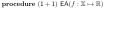
\includegraphics[width=0.75\paperwidth]{\sharedDir/graphics/metaheuristic_algorithms/opoea/opoea_1}}%
}{0.125}{0.445}%
%
\locate{3}{%
\algobox{0.75}{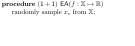
\includegraphics[width=0.75\paperwidth]{\sharedDir/graphics/metaheuristic_algorithms/opoea/opoea_2}}%
}{0.125}{0.445}%
%
\locate{4}{%
\algobox{0.75}{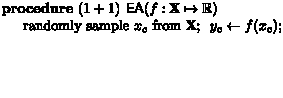
\includegraphics[width=0.75\paperwidth]{\sharedDir/graphics/metaheuristic_algorithms/opoea/opoea_3}}%
}{0.125}{0.445}%
%
\locate{5}{%
\algobox{0.75}{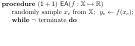
\includegraphics[width=0.75\paperwidth]{\sharedDir/graphics/metaheuristic_algorithms/opoea/opoea_4}}%
}{0.125}{0.445}%
%
\locate{6}{%
\algobox{0.75}{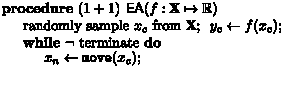
\includegraphics[width=0.75\paperwidth]{\sharedDir/graphics/metaheuristic_algorithms/opoea/opoea_5}}%
}{0.125}{0.445}%
%
\locate{7}{%
\algobox{0.75}{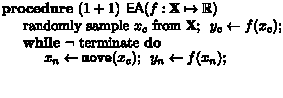
\includegraphics[width=0.75\paperwidth]{\sharedDir/graphics/metaheuristic_algorithms/opoea/opoea_6}}%
}{0.125}{0.445}%
%
\locate{8}{%
\algobox{0.75}{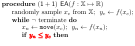
\includegraphics[width=0.75\paperwidth]{\sharedDir/graphics/metaheuristic_algorithms/opoea/opoea_7}}%
}{0.125}{0.445}%
%
\locate{9}{%
\algobox{0.75}{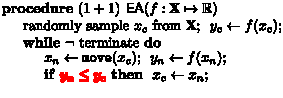
\includegraphics[width=0.75\paperwidth]{\sharedDir/graphics/metaheuristic_algorithms/opoea/opoea_8}}%
}{0.125}{0.445}%
%
\locate{10}{%
\algobox{0.75}{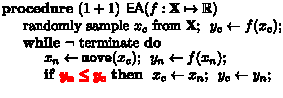
\includegraphics[width=0.75\paperwidth]{\sharedDir/graphics/metaheuristic_algorithms/opoea/opoea_9}}%
}{0.125}{0.445}%
%
\locate{11-}{%
\algobox{0.75}{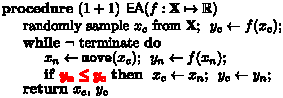
\includegraphics[width=0.75\paperwidth]{\sharedDir/graphics/metaheuristic_algorithms/opoea/opoea}}%
}{0.125}{0.445}%
%
\end{frame}%
%
\begin{frame}%
\frametitle{Research Field}%
\begin{itemize}%
%
\item My students and I together work on solving discrete or combinatorial problems with metaheuristic algorithms.%
%
\item<2-> We investigate classical hard problems that have discrete search spaces, such as bit strings or permutations.%
%
\item<3-> Here, the objective functions take on only natural numbers in~\naturalNumbersZ.%
%
\item<4-> We try to enable metaheuristic algorithms to find better solutions for these problems.%
%
\end{itemize}%
\end{frame}%
%
%
\section{Research Direction: \mbox{Frequency Fitness Assignment}}%
%
\begin{frame}%
\frametitle{Metaheuristic Optimization Algorithms}%
%
\begin{itemize}%
%
\item The most fundamental concept in metaheuristic optimization is%%
%
\end{itemize}%
%
\begin{center}\textbf{\large{\textcolor{red}{%
If you keep good solutions and modify them, you are likely to get better solutions.%
\uncover<2->{\medskip\\%
If you keep accepting better and better solutions, you will get really good solutions eventually.%
}%
}}}\end{center}%
%
\uncover<3->{%
\begin{itemize}%
\item<3-> Algorithms like random sampling or exhaustive enumeration that do not at least statistically prefer better solutions have extremely bad performance.%
%
\item<4-> We \alert{challenge} this principle.%
%
\item<5-> Our \glsFull{algoFFA} does \alert{\textbf{not}} prefer better solutions {\dots} yet it can improve the performance of existing algorithms in several cases!%
\end{itemize}}%
%
\end{frame}%
%
%
\begin{frame}%
\frametitle{FFA: Idea}%
\begin{itemize}%
\item \GlsFull{algoFFA} is a module that can be plugged into different existing algorithms.%
\item<2-> It changes the way the algorithm selects the interesting solutions~$S_{i+1}$ from the sets~$P_i=S_i\cup N_i$.%
\item<3-> It therefore maintains a table~$H$ with the encounter frequency of each objective value in the selection decisions.%
\item<4-> The table~$H$ is initially filled with zeros.%
\item<5-> Before the selection step of the algorithm, $H[f(P_i[j])]$ for all $j\in\intRange{1}{|P_i|}$ is incremented by~1.%
\item<6-> Then, the frequencies~$H[f(P_i[j])]$ replace the objective values $f(P_i[j])$ in the actual selection decisions.%
\end{itemize}%
\end{frame}%
%
\begin{frame}[t]%
\frametitle{FFA: (1+1)~EA and (1+1)~FEA}%
%
\begin{itemize}%
\only<-1>{%
\item Let's plug \gls{algoFFA} into the \gls{algoEAopo} and obtain the \glsFull{algoFEAopo}.%
}%
\only<-2>{%
\item<2-> We start with the \gls{algoEAopo}.%
}\only<-3>{%
\item<3-> We begin by initializing the frequency table~$H$ with all zeros.%
}\only<-4>{%
\item<4-> \emph{Before} the selection decision, we increment the frequency values of the objective values of all current solutions.%
}\only<-5>{%
\item<5-> Now the frequency values replace the objective values in the selection decisions.%
}%
\item<6-> Since we may now lose the best-so-far solution, we need to track it in additional variables.%
\item<8-> {\dots}which are then the return values of the \gls{algoFEAopo}.%
\end{itemize}%
%
\locate{}{%
\algobox{0.45}{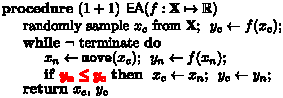
\includegraphics[width=0.45\paperwidth]{\sharedDir/graphics/metaheuristic_algorithms/opoea/opoea}}%
}{0.033333333}{0.4}%
%
%
\locate{2-}{%
\algobox{0.45}{%
\only<2>{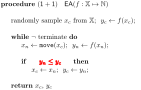
\includegraphics[width=0.45\paperwidth]{\sharedDir/graphics/metaheuristic_algorithms/fea/fea_1}}%
\only<3>{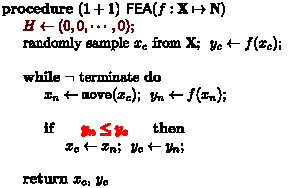
\includegraphics[width=0.45\paperwidth]{\sharedDir/graphics/metaheuristic_algorithms/fea/fea_2}}%
\only<4>{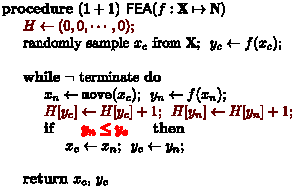
\includegraphics[width=0.45\paperwidth]{\sharedDir/graphics/metaheuristic_algorithms/fea/fea_3}}%
\only<5>{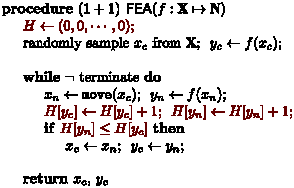
\includegraphics[width=0.45\paperwidth]{\sharedDir/graphics/metaheuristic_algorithms/fea/fea_4}}%
\only<6>{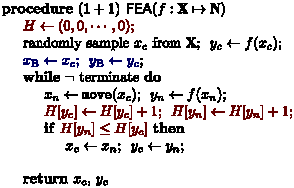
\includegraphics[width=0.45\paperwidth]{\sharedDir/graphics/metaheuristic_algorithms/fea/fea_5}}%
\only<7>{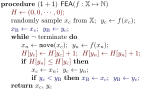
\includegraphics[width=0.45\paperwidth]{\sharedDir/graphics/metaheuristic_algorithms/fea/fea_6}}%
\only<8->{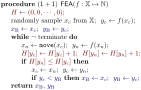
\includegraphics[width=0.45\paperwidth]{\sharedDir/graphics/metaheuristic_algorithms/fea/fea}}%
}%
}{0.516666666}{0.3}%
%
\end{frame}%
%
%
\begin{frame}%
\frametitle{FFA: What does this do?}%
\begin{itemize}%
\item The rating $H[f(x)]$ of a solution~$x$ depends only on how often solutions~$x'$ with $f(x')=f(x)$ have previously been seen in the optimization process.%
\item<2-> Static optimization problems become dynamic, because frequency fitness~$H$ changes over time.%
\item<3-> Solutions get less attractive the more often their corresponding objective values have been seen. This also holds for local optima\dots%
\item<4-> Solutions with better objective values are no longer preferred over such with worse objective value.%
\item<5-> Instead, solutions with less-frequent objective values are preferred.%
\item<6-> \alert{Algorithms using \gls{algoFFA} are invariant under all injective transformations of the objective function value.}%
\item<7-> They are less likely to get stuck at local optima, which is a problem for, e.g., the \gls{algoEAopo}.%
\end{itemize}%
\end{frame}%
%
\section{Our Results}%
%
\begin{frame}[t]%
\frametitle{Three Core Works}%
%
\locateGraphic{1-}{width=0.45\paperwidth}{\sharedDir/graphics/papers/WWWTDY2014FFA}{0.025}{0.15}%
\locateGraphic{2-}{width=0.45\paperwidth}{\sharedDir/graphics/papers/WWLC2021FFAMOAIUBTOTOFV}{0.275}{0.225}%
\locateGraphic{3-}{width=0.45\paperwidth}{\sharedDir/graphics/papers/WWLCL2023FFAOWBFGSCBE}{0.5}{0.3}%
%
\hspace{0.5\paperwidth}snippets of~\bracketCite{WWWTDY2014FFA,WWLC2021FFAMOAIUBTOTOFV,WWLCL2023FFAOWBFGSCBE}%
\end{frame}%
%
\begin{frame}[t]%
\frametitle{Discrete Benchmark Functions}%
%
\begin{itemize}%
%
\item Discrete optimization algorithms work on bit strings of length~$n$ as search space and use only the objective values of the solutions they sample to solve a problem.%
\end{itemize}%
%
\uncover<2->{\parbox{0.6\paperwidth}{%
\begin{itemize}%
%
\item They are usually tested on a variety of benchmark problems.%
%
\item<3-> We plug \pgls{algoFFA} into the \gls{algoEAopo} and obtain the \gls{algoFEAopo}.%
%
\item<4-> The \gls{algoEAopo} can easily solve the OneMax problem, where the goal is to find a bit string of all~\texttt{1}s\cite{M1992HGARWMAH}.%
%
\item<5-> It needs \bigThetab{n^n} on traps\cite{DJW2002OTAOTOPOEA}, where the optimum and the worst solution are exchanged compared to OneMax\only<-5>{.}\uncover<6->{, as well as on TwoMax\cite{FQW2018ELDBOAWHTMO,VHGN2002FTTIMEAHSP}, which has one local and one global optimum.}%
\end{itemize}}%
\uncover<7->{%
\begin{itemize}%
\item The \gls{algoFEAopo} solves all three problems in polynomial time\only<-7>{!}\uncover<8->{ as well as the Jump problem, where the \pgls{algoEAopo} also needs exponential runtime!}%
\end{itemize}}}%
%
\locateGraphic{4}{width=0.35\paperwidth}{\sharedDir/graphics/discrete_benchmarks/discrete_benchmarks_onemax}{0.63}{0.3}%
\locateGraphic{5}{width=0.35\paperwidth}{\sharedDir/graphics/discrete_benchmarks/discrete_benchmarks_onemax_trap}{0.63}{0.3}%
\locateGraphic{6}{width=0.35\paperwidth}{\sharedDir/graphics/discrete_benchmarks/discrete_benchmarks_twomax}{0.63}{0.3}%
\locateGraphic{8}{width=0.35\paperwidth}{\sharedDir/graphics/discrete_benchmarks/discrete_benchmarks_jump}{0.63}{0.3}%
%
\end{frame}%
%
\begin{frame}[t]%
\frametitle{Maximum Satisfiability Problem}%
\begin{itemize}%
\item \Gls{algoFFA} on the \glsFull{optMaxSAT} Problem, one of the most famous discrete optimization problems~\bracketCite{WWLCL2023FFAOWBFGSCBE,WWLC2021FFAMOAIUBTOTOFV,WWWTDY2014FFA}.%
\end{itemize}%
%
\uncover<2->{%
\vspace{-1em}%
\begin{center}%
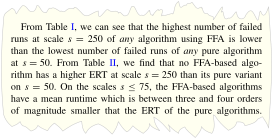
\includegraphics[width=0.6\paperwidth]{\sharedDir/graphics/papers/WWLCL2023FFAOWBFGSCBE_p10_snippet}%
\end{center}%
\vspace{-1em}%
%
\begin{itemize}%
\item Snippet of page~10 of~\bracketCite{WWLCL2023FFAOWBFGSCBE}~(copyright~IEEE).%
\item Several different \glspl{algoEA} with and without \gls{algoFFA}%
\end{itemize}%%
}%
%
\end{frame}%
%
\begin{frame}%
\frametitle{Traveling Salesperson Problem}%
\parbox{0.5\paperwidth}{%
\begin{itemize}%
\item \Gls{algoFFA} on the \glsFull{optTSP}:~\bracketCite{LWLvdBTW2024ATTSPWFFAAHA,LWLvdBW2022STTSPUFFA,LWTWW2024GSIWIFFTTSP}.%
\item<2-> Snippet of page~12 of~\bracketCite{LWLvdBTW2024ATTSPWFFAAHA}~(copyright Springer).%
\item<2-> \gls{algoEAopo}, \gls{algoFEAopo}, \glsFull{algoSA} w/o \gls{algoFFA}, hybrids%
\end{itemize}%
}%
%
\locateGraphic{2}{width=0.45\paperwidth}{\sharedDir/graphics/papers/LWLvdBTW2024ATTSPWFFAAHA_p12_snippet}{0.525}{0.03}%
\end{frame}%
%
\begin{frame}%
\frametitle{Quadratic Assignment Problem}%
\parbox{0.5\paperwidth}{%
\begin{itemize}%
\item \Gls{algoFFA} on the \glsFull{optQAP}:~\bracketCite{CWTW2024FFAOWBFGSORLSOTQAP,TOvdBLW2024ESTAEFFFA}.%
\item<2-> Snippet of page~7 of~\bracketCite{CWTW2024FFAOWBFGSORLSOTQAP}~(copyright SciTePress).%
\item<2-> \gls{algoRLS} w/o \gls{algoFFA}%
\end{itemize}%
}%
%
\locateGraphic{2}{width=0.45\paperwidth}{\sharedDir/graphics/papers/CWTW2024FFAOWBFGSORLSOTQAP_p7_snippet}{0.525}{0.03}%
%
\end{frame}%
%
\begin{frame}%
\frametitle{Job Shop Scheduling Problem}%
\begin{itemize}%
\item \Gls{algoFFA} on the \glsFull{optJSSP} Problem:~\bracketCite{WWLC2021FFAMOAIUBTOTOFV,WLCW2021SJSSPWUABFGS,dBTvdB2023FFAOJACR}.%
\end{itemize}%
%
\uncover<2->{%
\vspace{-1em}%
\begin{center}%
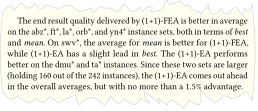
\includegraphics[width=0.6\paperwidth]{\sharedDir/graphics/papers/WLCW2021SJSSPWUABFGS_p4_snippet}%
\end{center}%
\vspace{-1em}%
%
\begin{itemize}%
\item Snippet of page~10 of~\bracketCite{WLCW2021SJSSPWUABFGS}~(copyright~ACM).%
\end{itemize}%%
}%
%
\end{frame}%
%
\begin{frame}%
\frametitle{Algorithm Synthesis and Genetic Programming}%
\begin{itemize}%
\item \Gls{algoFFA} for algorithm synthesis and \glsFull{algoGP}:~\bracketCite{WWTY2014EEIAWGP,WWWTDY2014FFA}.%
\end{itemize}%
%
\uncover<2->{%
\vspace{-1em}%
\begin{center}%

\includegraphics[width=0.6\paperwidth]{\sharedDir/graphics/papers/WWTY2014EEIAWGP_07_snippet}%
\end{center}%
\vspace{-1em}%
%
\begin{itemize}%
\item Snippet of page~7 of~\bracketCite{WWTY2014EEIAWGP}~(copyright~IEEE).%
\end{itemize}%%
}%
%
\end{frame}%
%
%
\section{Future Works}%
%
\begin{frame}%
\frametitle{Future Works}%
%
\begin{itemize}%
%
\item Apply \pgls{algoFFA} to other discrete and combinatorial problems\only<-1>{.}\uncover<2->{:%
\begin{enumerate}%
\item Where can \pgls{algoFFA} improve the solution quality?%
\item<3-> Where can it not do that?%
\item<4-> Why?%
\end{enumerate}%
}%
%
\item<5-> Plug \pgls{algoFFA} into more optimization algorithms.%
%
\item<6-> Combine \inQuotes{traditional} and \pgls{algoFFA}-based optimization, i.e., create hybrid algorithms, to reap the best of both worlds.%
%
\end{itemize}%
\end{frame}%
%
\section{Summary}%
%
\begin{frame}%
\frametitle{Summary}%
%
\begin{itemize}%
%
\item Our students and I work on the big field of optimization.%
%
\item<2-> We try to improve the quality of solutions that metaheuristics can deliver on discrete or combinatorial problems.%
%
\item<3-> We have a very interesting and novel technique called \glsFull{algoFFA}.%
%
\item<4-> We are figuring out where it really can give us better results.%
%
\item<5-> But we are not picky.\uncover<6->{ For example,%
\begin{enumerate}%
\item on the two-dimensional bin packing problem, we found out that a simple local search can actually \alert{outperform} the complex state-of-the-art metaheuristics and \pgls{algoFFA} could not improve the performance {\dots} so we published this surprising result and the student graduated with it\cite{ZLWvdBTW2024RLSOT2RBPPWIR,ZWvdBTLTW2024RLSFTDBPAANRFFFA}\only<-6>{.}\uncover<7->{, and}%
%
\item<7-> on the \glsFull{optTTP}, we also got surprisingly good results with \gls{algoRLS}\cite{XWvdBW2024RLSVNVFFAOTTTP} and \pgls{algoSA}.%
\end{enumerate}}%
%
\end{itemize}%
%
\end{frame}%
%
\section{Advertisement}%
%
\begin{frame}[t]%
\frametitle{Programming with Python}%
We have a freely available course book on \citetitle{programmingWithPython} at \citeurl{programmingWithPython}, with focus on practical software development using the \python\ ecosystem of tools\cite{programmingWithPython}.%
%
\locateGraphic{}{width=0.63\paperwidth}{\sharedDir/graphics/advertisement/snippets/programmingWithPythonSnippet}{0.025}{0.3}%
\locateGraphic{}{width=0.27\paperwidth}{\sharedDir/graphics/advertisement/urlQr/programmingWithPythonCourseUrl}{0.675}{0.4}%
%
\end{frame}%
%
\begin{frame}[t]%
\frametitle{Databases}%
We have a freely available course book on \citetitle{databases} at \citeurl{databases}, with actual practical examples using a real \dbms\cite{databases}.%
%
\locateGraphic{}{width=0.63\paperwidth}{\sharedDir/graphics/advertisement/snippets/databasesSnippet}{0.025}{0.3}%
\locateGraphic{}{width=0.27\paperwidth}{\sharedDir/graphics/advertisement/urlQr/databasesCourseUrl}{0.675}{0.4}%
%
\end{frame}%
%
%
\endPresentation%
\end{document}%%
\endinput%
%
